\chapter{मानव जनन}\label{ch:g5:human-reproduction}

तुम जिस भी व्यक्ति को जानते हो --- साथी, शिक्षक, अपने परिवार का सबसे
बुज़ुर्ग व्यक्ति --- वह इसी एक रास्ते से आया: शिशु के रूप में, अपनी माँ
के भीतर महीनों बढ़ने के बाद जन्म लेकर। मनुष्य \omterm{prop:g3:sorting-living-things:groups}{स्तनधारी} हैं
(\cref{prop:g4:classifying-animals:classes}), और मानव जनन
\cref{ch:g4:animal-reproduction} की \omterm{prop:g3:sorting-living-things:groups}{स्तनधारी} बनावट पर ही चलता है ---
बस उसमें हमारी अपनी \omterm{def:g5:biodiversity:species}{प्रजाति} की संख्याएँ, तारीख़ें और ब्यौरे जुड़े हैं,
जिन्हें यह अध्याय साफ़-साफ़ रखता है।

\section{इस बनावट का मानव रूप}

\begin{proposition}[मानव जनन स्तनधारी जनन है]\label{prop:g5:human-reproduction:plan}
सारे \omterm{prop:g3:sorting-living-things:groups}{स्तनधारियों} की तरह मनुष्य भी \omterm{def:g4:animal-reproduction:sexual}{लैंगिक जनन} करते हैं
(\cref{def:g4:animal-reproduction:sexual}):
\begin{itemize}
  \item माँ का शरीर \emph{\omterm{def:g4:animal-reproduction:sexual}{अंडाणु}} बनाता है; पिता का
        \emph{\omterm{def:g4:animal-reproduction:sexual}{शुक्राणु}};
  \item \omterm{def:g5:flower-to-fruit:steps}{निषेचन} --- यानी एक \omterm{def:g4:animal-reproduction:sexual}{शुक्राणु} का एक \omterm{def:g4:animal-reproduction:sexual}{अंडाणु} से जुड़ना ---
        \emph{माँ के शरीर के भीतर} होता है
        (\cref{prop:g4:animal-reproduction:where});
  \item निषेचित \omterm{def:g4:animal-reproduction:sexual}{अंडाणु} --- एक अकेली \omterm{def:g5:first-look-at-cells:cell}{कोशिका}
        (\cref{ex:g5:first-look-at-cells:one}) --- माँ के
        \emph{गर्भाशय}\index{गर्भाशय} में जम जाता है और वहीं बढ़ता है;
  \item मनुष्य \omterm{def:g4:animal-reproduction:ovivivi}{जरायुज} हैं
        (\cref{def:g4:animal-reproduction:ovivivi}): शिशु \omterm{def:g2:animals-grow-up:born}{जीवित जन्म}
        लेता है, और शुरू में \omterm{def:g2:animals-grow-up:born}{दूध} पर पलता है।
\end{itemize}
\end{proposition}
\admitted

\begin{remark}[जनन के लिए वयस्क शरीर चाहिए]\label{rem:g5:human-reproduction:adults}
बच्चे का शरीर बच्चे नहीं कर सकता: जननिक अंग \emph{यौवनारंभ} पर ही काम
करना शुरू करते हैं, यानी \cref{def:g3:stages-of-life:stages} की \omterm{def:g3:stages-of-life:stages}{किशोर}
अवस्था वाले उस बदलाव पर, जब शरीर अपने को बालक के शरीर से वयस्क के शरीर
में फिर से गढ़ता है। यौवनारंभ क्या-क्या बदलता है और कैसे, यह इस पुस्तक
के माध्यमिक वर्षों के एक पूरे अध्याय का विषय है।
\end{remark}

\section{गर्भाशय में नौ महीने}

\begin{definition}[गर्भावस्था]\label{def:g5:human-reproduction:pregnancy}
\emph{गर्भावस्था}\index{गर्भावस्था} वह समय है जो भावी शिशु अपनी माँ के
\omterm{prop:g5:human-reproduction:plan}{गर्भाशय} में बढ़ते हुए बिताता है: मनुष्यों में लगभग \emph{नौ महीने}।
बढ़ते हुए शिशु को पहले \emph{भ्रूण}\index{भ्रूण} कहते हैं, और फिर ---
लगभग दो महीने बाद, जब उसके शरीर की बनावट तय हो जाती है ---
\emph{गर्भस्थ शिशु}\index{गर्भस्थ शिशु}।
\end{definition}

\begin{proposition}[नाल के ज़रिए पोषण]\label{prop:g5:human-reproduction:cord}
\omterm{prop:g5:human-reproduction:plan}{गर्भाशय} के भीतर शिशु तरल की एक थैली में तैरता है और न खा सकता है, न
साँस ले सकता है। सब कुछ माँ के \omterm{prop:g4:journey-of-food:absorb}{रक्त} से बना-बनाया आता है: \omterm{def:g4:journey-of-food:digestion}{पोषक तत्व} और
ऑक्सीजन (\cref{prop:g4:heart-and-blood:carries}) उसके पेट पर लगी
\emph{नाभि-रज्जु}\index{नाभि-रज्जु} से होकर शिशु के \omterm{prop:g4:journey-of-food:absorb}{रक्त} में उतरते हैं
--- और उसका कचरा उसी रास्ते वापस जाता है, ताकि माँ का शरीर उसे सँभाल
ले। तुम्हारी नाभि वही जगह है जहाँ तुम्हारी अपनी नाल जुड़ी थी।
\end{proposition}
\admitted

\begin{example}[नौ महीने का समय-पत्रक]\label{ex:g5:human-reproduction:timetable}
पहला महीना: बँटती \omterm{def:g5:first-look-at-cells:cell}{कोशिकाओं} का एक गुच्छा, चावल के दाने से भी छोटा, पर
पहले से तेज़ी से बढ़ता हुआ। दूसरा महीना: एक \omterm{def:g5:human-reproduction:pregnancy}{भ्रूण}, जिसमें \omterm{def:g1:my-body:parts}{सिर} का ख़ाका,
धड़कता \omterm{def:g4:heart-and-blood:heart}{हृदय}, और \omterm{def:g1:my-body:parts}{बाँहों} तथा \omterm{def:g1:my-body:parts}{टाँगों} की कलियाँ हैं --- और जो अब भी अँगूठे
से छोटा है। तीसरा-चौथा महीना: एक \omterm{def:g5:human-reproduction:pregnancy}{गर्भस्थ शिशु}, बनावट में पूरा, जो हिलना
शुरू कर देता है; माँ को जल्द ही उसकी ठोकरें महसूस होने लगती हैं।
पाँचवाँ से आठवाँ महीना: बढ़ना और पकना --- सुनना आ जाता है, और बालों की
पहली परत भी। नौवाँ महीना: शिशु, आम तौर पर \omterm{def:g1:my-body:parts}{सिर} नीचे किए और लगभग
\qty{3}{kg} का, तैयार है।
\end{example}

\begin{example}[जन्म]\label{ex:g5:human-reproduction:birth}
जन्म के समय \omterm{prop:g5:human-reproduction:plan}{गर्भाशय} की ताक़तवर \omterm{def:g3:bones-and-muscles:muscle}{पेशियाँ} शिशु को दुनिया में धकेल देती
हैं, आम तौर पर \omterm{def:g1:my-body:parts}{सिर} पहले। पहली किलकारी फेफड़ों को हवा से भर देती है ---
उन्होंने पहले कभी साँस ली ही नहीं थी
(\cref{prop:g5:human-reproduction:cord}) --- नाल, जिसकी अब ज़रूरत नहीं,
बिना दर्द के काट दी जाती है, और \omterm{prop:g3:sorting-living-things:groups}{स्तनधारी} बनावट बाहर भी चलती रहती है:
\omterm{def:g2:animals-grow-up:born}{दूध}, गरमाहट और देखभाल (\cref{ex:g4:animal-reproduction:whalecalf}
इससे सहमत होता)।
\end{example}

\begin{omfigure}
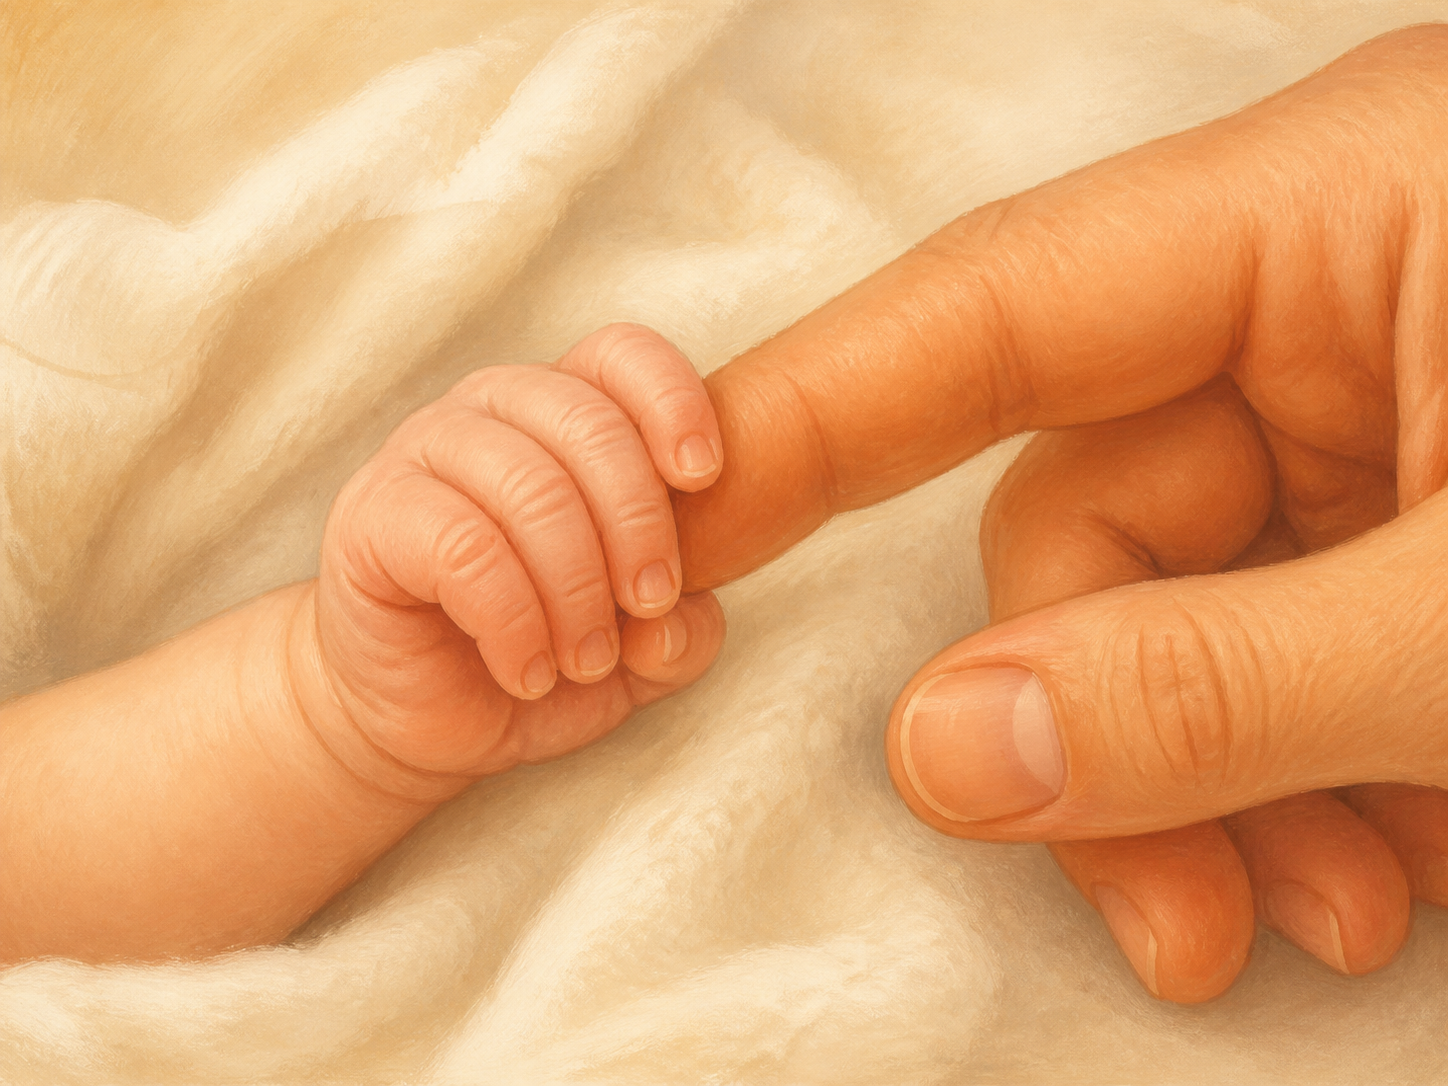
\includegraphics[width=0.52\linewidth]{images/book1/ai/g5-human-babyhand.png}

{\small कुछ ही दिन का, और पकड़ अभी से काम कर रही है: मनुष्य का लंबा
बचपन शुरू होता है।}
\end{omfigure}

\begin{remark}[जुड़वाँ]\label{rem:g5:human-reproduction:twins}
कभी-कभी \omterm{prop:g5:human-reproduction:plan}{गर्भाशय} में दो शिशु साथ-साथ बढ़ते हैं। अगर एक निषेचित \omterm{def:g4:animal-reproduction:sexual}{अंडाणु}
बँटकर दो \omterm{def:g5:human-reproduction:pregnancy}{भ्रूण} बन गया हो, तो जुड़वाँ \emph{एकसमान} होते हैं --- एक ही
शुरुआती \omterm{def:g5:first-look-at-cells:cell}{कोशिका} से बने, दो नक़लों जैसे मिलते-जुलते। और अगर दो \omterm{def:g4:animal-reproduction:sexual}{अंडाणु} दो
शुक्राणुओं से निषेचित हुए हों, तो जुड़वाँ आम भाई-बहनों से ज़्यादा एक
जैसे नहीं होते --- उन्होंने बस \omterm{prop:g5:human-reproduction:plan}{गर्भाशय} साझा किया था। दो तरह के जुड़वाँ,
जिन्हें उनकी शुरुआत से पहचाना जाता है।
\end{remark}

\section{पहले और बाद की देखभाल}

\begin{proposition}[शिशु अपनी माँ की आपूर्ति बाँटता है]\label{prop:g5:human-reproduction:care}
शिशु तक जो कुछ पहुँचता है वह माँ के \omterm{prop:g4:journey-of-food:absorb}{रक्त} से होकर आता है --- इसीलिए
गर्भवती माँ अच्छा खाती है (\cref{ch:g3:balanced-diet}), आराम करती है,
डॉक्टरों या दाइयों की देखरेख में रहती है, और उन चीज़ों से बचती है जो
शिशु को नुक़सान पहुँचा सकती हैं: तंबाकू का धुआँ और शराब भी नाल से होकर
गुज़र जाते हैं, और \omterm{def:g5:human-reproduction:pregnancy}{गर्भस्थ शिशु} वयस्क से कहीं ज़्यादा नाज़ुक होता है।
माँ की देखभाल \emph{ही} शिशु की देखभाल है।
\end{proposition}
\admitted

\begin{example}[बहुत देखभाल वाली एक प्रजाति]\label{ex:g5:human-reproduction:longcare}
\omterm{prop:g3:sorting-living-things:groups}{स्तनधारियों} में भी मनुष्य
\cref{prop:g4:animal-reproduction:strategies} की
कम-और-देखभाल-वाली रणनीति को सिरे तक ले जाते हैं: आम तौर पर एक बार में
एक शिशु, जो बछेड़े या बिल्ली के बच्चे से कहीं ज़्यादा देर तक असहाय रहता
है, और जिसकी --- खिलाकर, सिखाकर, प्यार करके --- कई \emph{सालों} तक
देखभाल की जाती है। मानव बचपन जंतु-जगत के सबसे लंबे बचपनों में से एक है;
और दस साल लंबा यह पाठ्यक्रम, यह पुस्तक, ख़ुद उसी लंबी देखभाल का एक
टुकड़ा है।
\end{example}

\section{अभ्यास}

\begin{exercise}[$\star$]\label{exo:g5:human-reproduction:1}
कौन-सी \omterm{def:g5:first-look-at-cells:cell}{कोशिका} माँ से आती है, कौन-सी पिता से, और उनके जुड़ने को क्या
कहते हैं?
\end{exercise}

\begin{exercise}[$\star$]\label{exo:g5:human-reproduction:2}
मानव शिशु कहाँ बढ़ता है, और लगभग कितने समय तक?
\end{exercise}

\begin{exercise}[$\star$]\label{exo:g5:human-reproduction:3}
बढ़ते शिशु के दोनों नाम क्रम से बताओ, और मोटे तौर पर यह भी कि पहला
दूसरा कब बनता है।
\end{exercise}

\begin{exercise}[$\star$]\label{exo:g5:human-reproduction:4}
\omterm{prop:g5:human-reproduction:plan}{गर्भाशय} में शिशु न खाता है न साँस लेता है। उसे \omterm{def:g4:journey-of-food:digestion}{पोषक तत्व} और ऑक्सीजन
कैसे मिलते हैं, और उसका कचरा कहाँ जाता है?
\end{exercise}

\begin{exercise}[$\star$]\label{exo:g5:human-reproduction:5}
तुम्हारी नाभि किस चीज़ का निशान है?
\end{exercise}

\begin{exercise}[$\star$]\label{exo:g5:human-reproduction:6}
पहली किलकारी पर क्या होता है, और यह शिशु के शरीर के लिए इतना बड़ा
बदलाव क्यों है?
\end{exercise}

\begin{exercise}[$\star$]\label{exo:g5:human-reproduction:7}
कौन-सी ख़ासियतें मानव जनन को ठेठ \omterm{prop:g3:sorting-living-things:groups}{स्तनधारी} बनाती हैं?
\cref{prop:g4:classifying-animals:classes} या
\cref{ch:g4:animal-reproduction} का हवाला देते हुए तीन बताओ।
\end{exercise}

\begin{exercise}[$\star$]\label{exo:g5:human-reproduction:8}
डॉक्टर गर्भवती माँओं से तंबाकू के धुएँ और शराब से बचने को क्यों कहते
हैं? \cref{prop:g5:human-reproduction:care} का इस्तेमाल करो।
\end{exercise}

\begin{exercise}[$\star\star$]\label{exo:g5:human-reproduction:9}
दोनों तरह के जुड़वाँओं को उनकी शुरुआत से समझाओ। कौन-सा जोड़ा ``दो
नक़लों जैसा'' मिलता-जुलता है, और यह
\cref{ex:g5:first-look-at-cells:one} से क्यों निकलता है?
\end{exercise}

\begin{exercise}[$\star\star$]\label{exo:g5:human-reproduction:10}
\cref{prop:g4:animal-reproduction:strategies} की रणनीति-रेखा पर मनुष्य
को रखो, और कॉड मछली तथा हाथी से तुलना करो: बच्चों की संख्या, देखभाल की
लंबाई, और मनुष्यों के लिए उस लंबी देखभाल में क्या-क्या शामिल है।
\end{exercise}

\begin{exercise}[$\star\star\star$]\label{exo:g5:human-reproduction:11}
जन्म के समय कटी हुई नाल शिशु की आपूर्ति-लाइन ठीक उसी क्षण ख़त्म कर
देती है जब \omterm{def:g4:breathing:organs}{फेफड़े} अपनी पहली साँस लेते हैं।
\cref{prop:g5:human-reproduction:cord} और
\cref{prop:g4:breathing:exchange} की मदद से समझाओ कि उस एक मिनट में
कौन-सा काम माँ के शरीर से शिशु के अपने फेफड़ों को सौंपा जाता है ---
और पहली किलकारी का समय इतना सही क्यों है।
\end{exercise}
